
\documentclass[conference]{IEEEtran}


\ifCLASSINFOpdf
  \usepackage{listings}
  \usepackage[pdftex]{graphicx}
  \usepackage{url}
  % \usepackage{caption}
  \usepackage{subcaption}
  \usepackage{tikz,pgfplots,pgfplotstable}
  \usepgfplotslibrary{statistics}

\else
\fi
\hyphenation{op-tical net-works semi-conduc-tor}


\begin{document}
\title{How Important are Usage Examples in REST API Documentation?}

\author{\IEEEauthorblockN{S M Sohan, Frank Maurer\IEEEauthorrefmark{1}}
\IEEEauthorblockA{\IEEEauthorrefmark{1}
Dept. of Computer Science\\
University of Calgary\\
Canada\\
\{smsohan, frank.maurer\}@ucalgary.ca}
\and
\IEEEauthorblockN{Craig Anslow}
\IEEEauthorblockA{School of Eng. and Computer Science\\
Victoria University of Wellington\\
New Zealand\\
craig@ecs.vuw.ac.nz}
\and
\IEEEauthorblockN{Martin Robillard}
\IEEEauthorblockA{
School of Computer Science\\
McGill University\\
Canada\\
martin@cs.mcgill.ca}
}

\maketitle

\begin{abstract}
Generating and maintaining REST API documentation with usage examples can be a time consuming and expensive process for evolving APIs. Most REST API documentation tools focus on automating the documentation of the API objects, but require manual effort for capturing realistic usage examples. So, REST API developers need to know the cost vs. benefit of providing usage examples in the documentation as well as what to include in the usage examples to prioritize the documentation efforts. In this paper, we present our observations about the obstacles that REST API client developers face without usage examples in the documentation. To this regard, we have performed a controlled study with 26 experienced software engineers and found that REST API client developers face productivity problems with using correct data types, data formats, required HTTP headers and request body when documentation lacks usage examples. By following the REST API documentation guidelines from this paper, practitioners can reduce the errors, improve success rate and satisfaction of REST API client developers.


\end{abstract}


\IEEEpeerreviewmaketitle

\section{Introduction}
Researchers have emphasized API documentation as key factor that impacts API usability both positively and negatively. To improve API documentation, researchers have recommended incorporating usage examples in the API documentation. REST APIs are used as the predominant application integration mechanism over the Internet. Generating and maintaining REST API documentation with usage examples can be an expensive process because most API documentation tools have a lack of support for capturing realistic usage examples.

In a resource constrained environment, it is important to understand the value of usage examples on REST API usability to allocate sufficient attention and efforts towards incorporating examples in the API documentation. While it is no surprise that examples help API client developers, REST API developers need to know what to include in the examples and why. To our knowledge, there's a lack of published papers that investigated the impact of different types of content that can be included as usage examples in REST API documentation.

The documentation of REST APIs has distinctive features compared to the documentation of local APIs such as Java libraries. For example, local API documentation commonly comprises of describing the modules, classes and interfaces with their methods. On the other hand, REST API documentation needs to include information about HTTP headers, request and response body and the data representation formats such as JSON, XML, etc. In our work we have focused on understanding the impact of usage examples within the realm of the distinctive REST API features.

We have designed and performed a controlled study with experienced software engineers. Participants were divided into two groups and given the same set of API tasks to complete. One group was given the official WordPress REST API documentation and another group was given a forked version of the documentation where three usage examples were added. Using a novel technique, we have collected 539 API calls made by the participants. We have analyzed the data and observed recurring obstacles faced by the participants while performing the API tasks using the official documentation that lacks usage examples. Our contributions on this paper is as follows:

\begin{itemize}
  \item We provide a list of obstacles that REST API client developers face while performing API tasks using documentation that lacks usage examples.
  \item We provide a list of recommendations for REST developers to be used as a guideline to incorporate usage examples in the API documentation.
  \item We provide an empirical evidence that usage examples in REST API documentation helps API client developers perform API tasks with higher developer satisfaction, less time, and better success rate.
\end{itemize}

The remainder of this paper is organized as follows: In Section \ref{sec:method} we discuss our research goals, requirements, the object of the study and the participant selection, the study setup, data collection and analysis methods. In Section \ref{sec:results} we discuss the results of our analysis. We discuss the threats to validity and provide a summary of the related work in Sections \ref{sec:threat} and  \ref{sec:related_work} respectively.

\section{Methodology}
\label{sec:method}
\subsection{Research Goals}
This research is aimed at answering the following research questions:

\begin{itemize}
  \item \textbf{RQ}. What obstacles API client developers face when using a REST API documentation that lacks usage examples?
\end{itemize}

\subsection{Requirements} % (fold)

To answer the aforementioned research questions, the study has the following requirements:

\begin{itemize}
  \item \textbf{R1. Representative API.} We had to choose an existing REST API that is currently used by API client developers. Selecting a mature REST API for this study reduces the possibility of an underdeveloped solution that may be found if a new or a seldom used API is selected. A familiar domain needed to be selected so that participants are able to relate to the API features without requiring upfront training. In addition to selecting the API, we had to select tasks that are related to the core features provided by the API to represent reality.
  \item \textbf{R2. Open source.} To be able to understand the impact of usage examples, we needed to select an open-source API where we can add new examples to the documentation for performing this study. For proprietary APIs, it won't be possible to retrofit usage examples on existing API documentation without separating the examples from the documentation.
  \item \textbf{R3. Time bound.} The total time spent by each participant is required to be time bound to measure productivity. As a result, the study needs to be setup such that participants are able to focus on performing the tasks minimizing any overhead.
  \item \textbf{R4. Experienced developers.} Developers with prior experience on REST APIs need to be recruited as study participants to perform the study within a limited amount of time and in a realistic setup. Furthermore, to reduce a learning bias, only participants with no prior experince of using the WordPress REST API V2 are accepted for this study.
\end{itemize}


\subsection{Study API} % (fold)

We selected the WordPress REST API V2 for this study. WordPress is a blog-like open-source (R2) framework used by over 409 million people to visit 23.6 billion pages each month. The API allows programmatic access to list, create, update, and delete WordPress data such as blog posts, comments, users, images, tags, etc.

The WordPress REST API V2 has been published and maintained since May 2015. Before January 2017, the WordPress REST API V2 was distributed as a plug-in where WordPress users could optionally install the API component. The following statistics are for the plug-in install numbers between May 2015 and October 2016:

\begin{itemize}
  \item Total installs: aprox. 248K installs of the plug-in.
  \item Average daily installs: approx. 500.
\end{itemize}

Starting January 2017, the WordPress REST API V2 is no longer required to be installed as a separate plug-in since it's pre-bundled with every WordPress install. As per the code repository on GitHub, there are a total of 99 and 46 contributors that had at least one commit to the code repository behind the API and and it's documentation, respectively. These properties satisfy R1, our requirements for using a representative API.

By selecting an open-source project we are able to access the source-code to inspect the implementation and documentation technique of the WordPress REST API. The API implements a self-documenting feature where API developers expose API endpoints over HTTP OPTIONS verb to explain the API elements. To implement this feature, the API developers describe the API elements in the code. For example:


\lstset{basicstyle=\footnotesize}
\begin{lstlisting}[language=php,breaklines=true,showspaces=false,showstringspaces=false,numbers=left,xleftmargin=2em,caption={Example of self-documenting API Code},label=wordpress_code]
public function get_item_schema() {
  $schema = array(
    '$schema'    => 'http://json-schema.org/draft-04/schema#',
    'title'      => $this->post_type,
    'type'       => 'object',
    /*
     * Base properties for every Post.
     */
    'properties' => array(
        'date'            => array(
            'description' => __( "The date the object was published, in the site's timezone." ),
            'type'        => 'string',
            'format'      => 'date-time',
            'context'     => array( 'view', 'edit', 'embed' ),
        ),...
\end{lstlisting}

On Listing \ref{wordpress_code}, line 4 specifies that this is a schema definition for the API element $Post$. Then, on Line 10, it defines $date$, one of the properties of $Post$, followed by a human readable description and and type information. Then, on line 14, the context of this property is mentioned as $view, edit, embed$, meaning that this property will be returned when the $Post$ object is returned, embedded, or can be used as an input for editing.

This self-documenting feature is leveraged to generate and publish the official API documentation as an HTML website. Figure \ref{fig:schema} shows a screenshot of the published documentation for the $date$ attribute of the $Post$ API element\footnote{\url{http://v2.wp-api.org/reference/posts/}}.

\begin{figure}[h!]
\begin{center}
\fbox{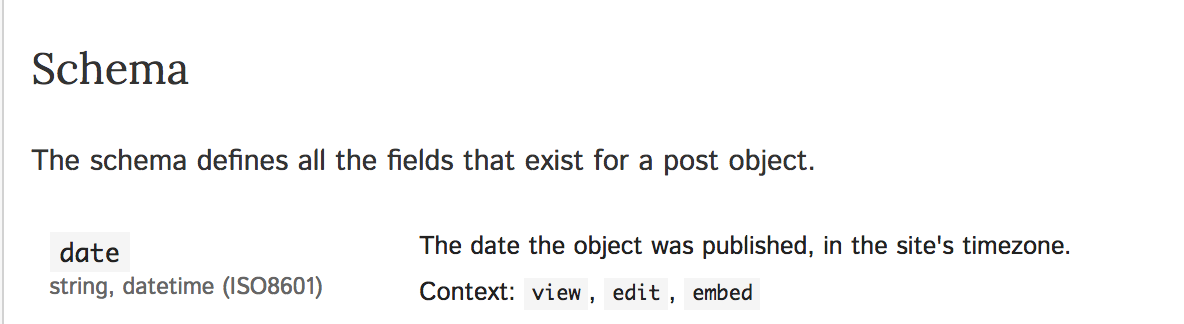
\includegraphics[width=\linewidth,keepaspectratio]{schema.png}}
\end{center}
\caption{Screenshot showing auto-generated documentation for Post/date}
\label{fig:schema}
\end{figure}

In addition to the auto-generated documentation of the the schema and API actions, custom content is added by the contributors to the API documentation project to provide prosaic overviews and usage examples.



\subsection{Study Design} % (fold)
\subsubsection{Tasks} % (fold)

The participants are requested to perform a total of six tasks using the API including one practice task. All of the tasks are related to a single API element, $Post$. The tasks get progressively difficult, and all but the last task can be performed independently of each other. Participants are requested to limit the total time on the study to a maximum of one hour. Participants are encouraged to proceed to the next task when they are either satisfied about or stuck on the right answer.

To use a REST API, the API client developers need to work with the following four inputs over HTTP:

\begin{itemize}
  \item I1. Request method
  \item I2. Request URL
  \item I3. Request headers
  \item I4. Request body
\end{itemize}

To verify the response of an API call, the API client developers can use HTTP response headers and/or HTTP response body. To perform the tasks, the participants are required to use one or more of the inputs I1-4. In the following paragraphs, we describe each task with it's description and the intended test scenario against the aforementioned API input and output information. For each of the tasks, the participants are required to use the same WordPress REST API and its documentation.

\textbf{T1: ListAllPostsTask}. We ask the participants to use the WordPress REST API following its documentation to get a list of the blog posts from a live WordPress site. This is the practice task, and the inputs to answer this task are pre-filled for the participants. It allows the participants to understand the tools used for this study as well as get familiarity with the Post API. The answer for this task makes use of I1 and I2.

\textbf{T2: FilterPostsByAuthorTask.} The participants are asked to use the API to filter the list of posts by an author given the author's user name. To answer this correctly, the participants are required to first make an API call to get the numeric ID of the author given the string based user name. Then, the ID needs to be used on the Post API to filter posts by the author. This task allows us to understand the impact of usage examples on API client developers when multiple API calls need to be made to perform a task using the API. Inputs I1-2 are required to complete this task successfully.

\textbf{T3: ExcludePostsByIdsTask.} We ask the participants to use the API to get a list of all posts excluding posts with IDs 1 and 4. Participants need to use the inputs I1-2, and use a desired format on I2 to pass an array of IDs as a parameter. This task allows us to understand how API client developers identify the format for using an array within the URL with respect to the usage examples in the API documentation.

\textbf{T4: FindTotalPostsTasks.} This task requires the participants to use the API to find a total number of posts. Participants need to use the inputs I1-2 and inspect the HTTP response headers to successfully complete this task. This task allows us to understand how API client developer productivity is affected with respect to missing examples about HTTP response headers in the API documentation.

\textbf{T5: PublishPostTask.} We ask the participants to use the API to publish a blog post with a specific title, content, and a published date. To successfully complete this task, the participants are required to use all four input types and inspect both the HTTP response header and the response body. Additionally, the participants are required to use a specific date format that the API accepts as a valid format for date specification. Answers to this task allows us to study API client developer productivity with respect to the usage examples lacking details about the inputs I3-4.

\textbf{T6: UpdatePostTask.} We ask the participants to use the API to update a blog post that they published in T5 with a new excerpt. Similar to T5, this task requires the use of inputs I1-4, but with different values for the inputs. This task allows us to understand API client developer productivity on inter-dependent tasks with respect to usage examples.

To summarize, the tasks allow us to understand how REST API client developers approach API tasks of different complexity levels involving various input types and available output information with respect to the usage examples in the API documentation.

\subsubsection{Participant Selection} % (fold)

To satisfy the requirement of developers with REST API experience (R3), we have used the following criteria for recruiting the study participants:

\begin{itemize}
  \item Currently working as a software engineer.
  \item At least 1 year of industry experience as a software engineer.
  \item At least 1 year of industry experience with REST APIs.
  \item No prior experience with WordPress REST API.
\end{itemize}

A total 26 participants from sixteen different companies and six different countries (Canada, USA, Germany, Ireland, Brazil, and,
Bangladesh) were recruited through online announcements posted on Twitter, Facebook, and software developer focused mailing lists. Table \ref{table:participants} shows a summary of the experience level of the participants on each group.

\begin{table}[!tbh]
  \caption{Participant Profile}
  \label{table:participants}

\begin{tabular}{|p{0.8in} p{.6in} p{0.7in} p{0.7in}|}

\hline
& & \textbf{Group 1} & \textbf{Group 2}\\
\hline
\multicolumn{2}{|l}{\textbf{Number of Participants}} & 16 (P1.1-P1.16) & 10 (P2.1-P2.10) \\
\hline
\multicolumn{4}{|l|}{\textbf{Industry Experience}} \\
& 1-5 years & 5 & 1 \\
& 5-10 years & 6 & 5 \\
& 10+ years & 5 & 4 \\
& Average & 9.1 & 10.6 \\
\hline

\multicolumn{4}{|l|}{\textbf{REST API Experience}} \\
&   1-3 years & 5 & 3 \\
&   3-5 years & 7 & 4 \\
&   5+ years & 4 & 3 \\
&   Average & 4.5 & 4 \\

\hline
\multicolumn{2}{|l}{\textbf{Number of Companies}} & 10 & 8 \\
\hline
\end{tabular}

\end{table}


\subsubsection{Process}

Two pilot studies were performed to evaluate and understand an effective process for performing this study. The first pilot study involved four participants that were invited to join the first author on this paper in-person or using a video conferencing software. The study involved tasks using two APIs, the WordPress REST API V2 and the GMail REST API. Each participant was given one of the two APIs and a set of tasks to complete using the API within an hour. Participants were given an online answer form to record the answers to the tasks. The primary findings from this pilot are as follows: 1) asking participants to use an API to perform the tasks required significant overhead time for them to setup a development environment with the proper API credentials, 2) the intermediate trial attempts of using the API are potentially more valuable than the final answer as it allows us to understand API client developer information needs that may are not answered by the documentation, 3) the number of tasks for the study had to be reduced so the participants could complete the tasks within the one hour limit, and 4) for GMail API, participants used up a large portion of their time on setting up their API credentials that requires understanding of OAuth.


\begin{figure*}[t]
\begin{center}
\fbox{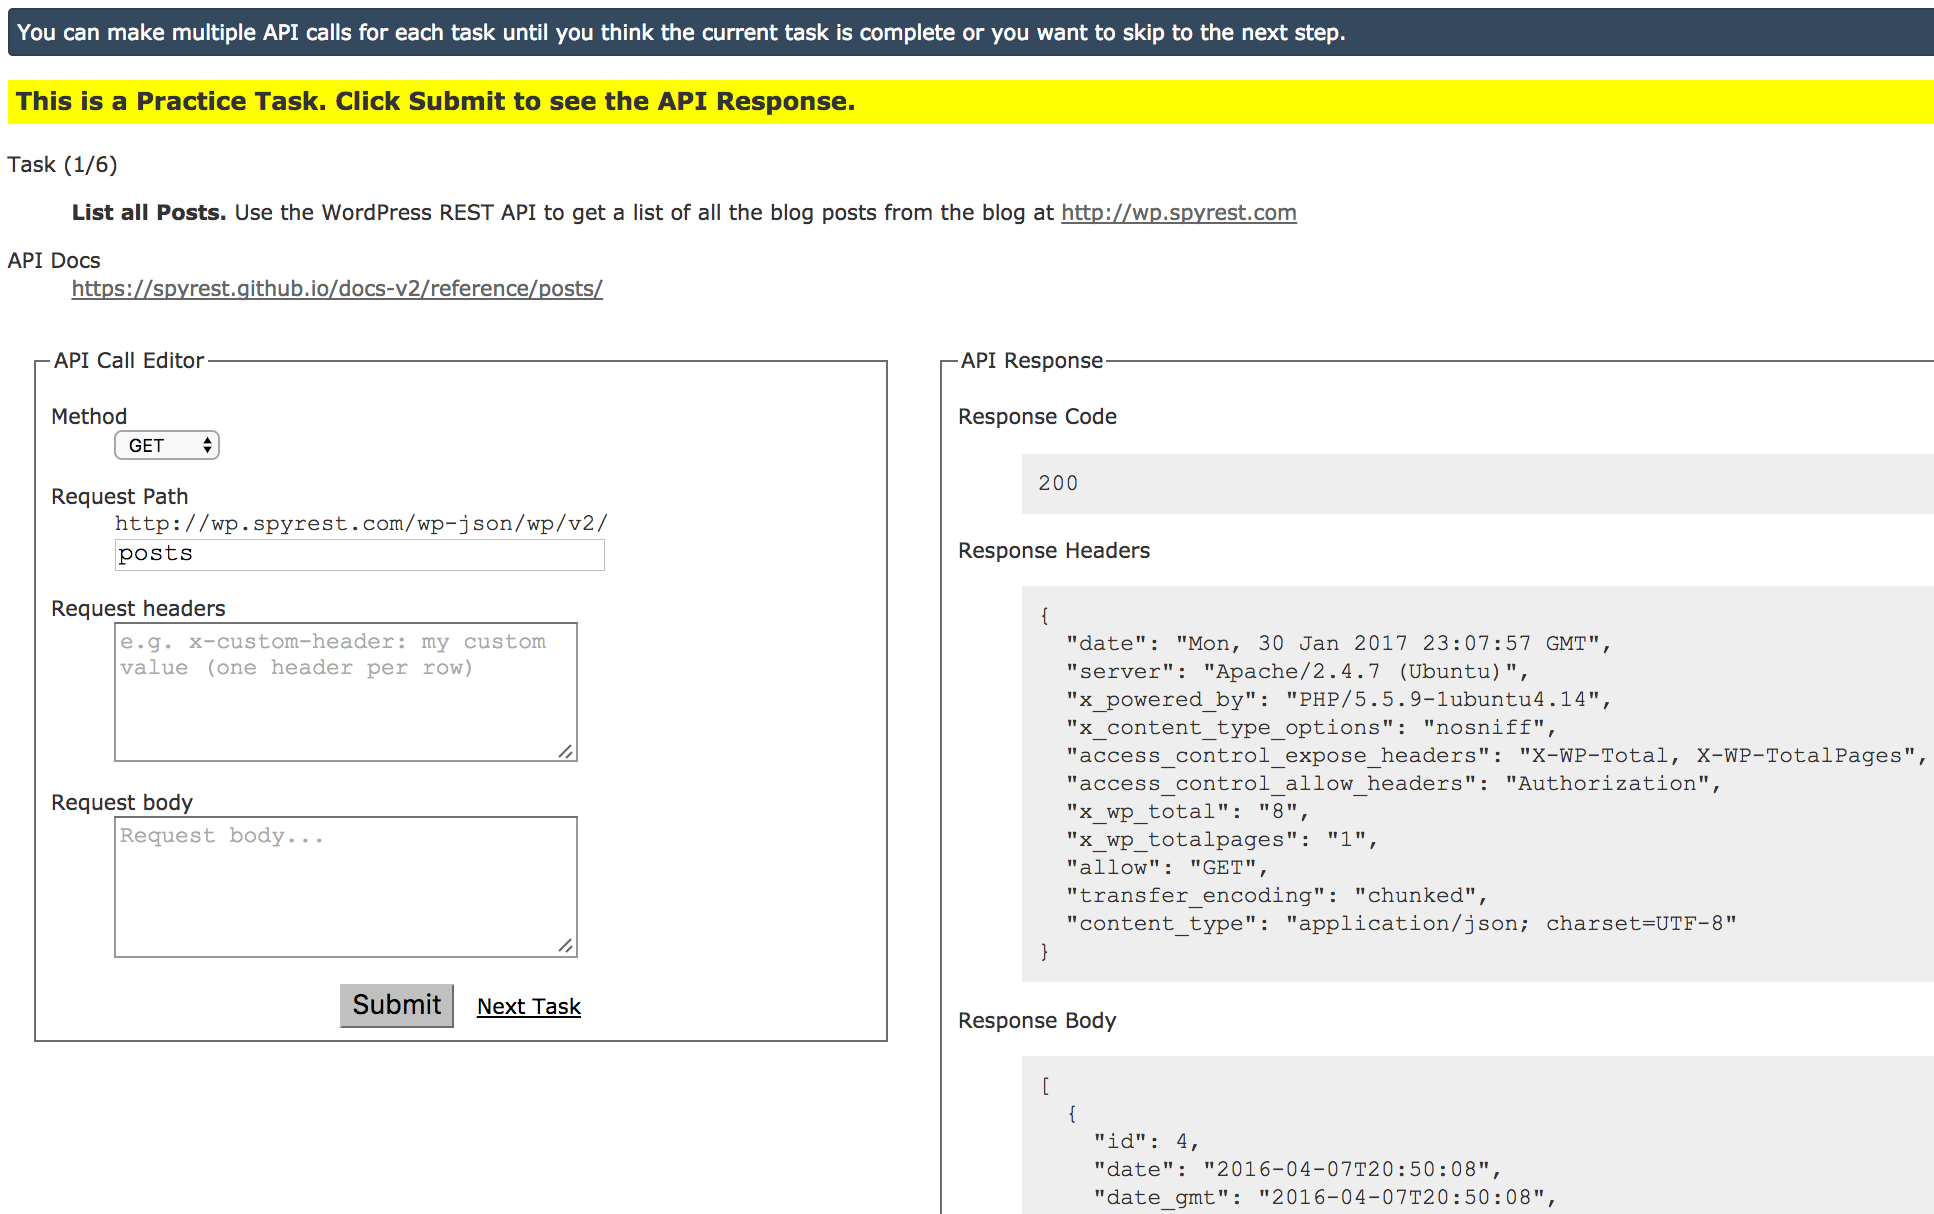
\includegraphics[width=\linewidth,keepaspectratio]{api_explorer.png}}
\end{center}
\caption{Screenshot of the web-based REST API explorer}
\label{fig:api_explorer}
\end{figure*}

To overcome the shortcomings found from the first pilot study, we decided to develop a web-based REST API explorer as shown on Figure \ref{fig:api_explorer} that allows participants to use their browser to make the API calls without setting up any development environment. The web-based API explorer only requires the inputs I1-4, and displays the HTTP response headers and body on the click of a button. Thus the participants could focus on using the right input and verifying the output without having to write any code. The web-base REST API explorer also allowed us to automatically collect all the trial API calls that the participants make for each API task. A second pilot study involving seven new participants was performed to understand the features of the web-based REST API explorer in practice and to improve the user interface based on feedback from the participants. Participants completed the study on their own without having to meet in-person or over video conferencing. Only the WordPress REST API was used to focus on REST APIs without the required learning curve associated with OAuth. We found encouraging results from this pilot study as the collected data showed patterns of mistakes that API client developers make that can be reduced by adding usage examples in the API documentation.


\begin{figure*}[t]
\begin{center}
\fbox{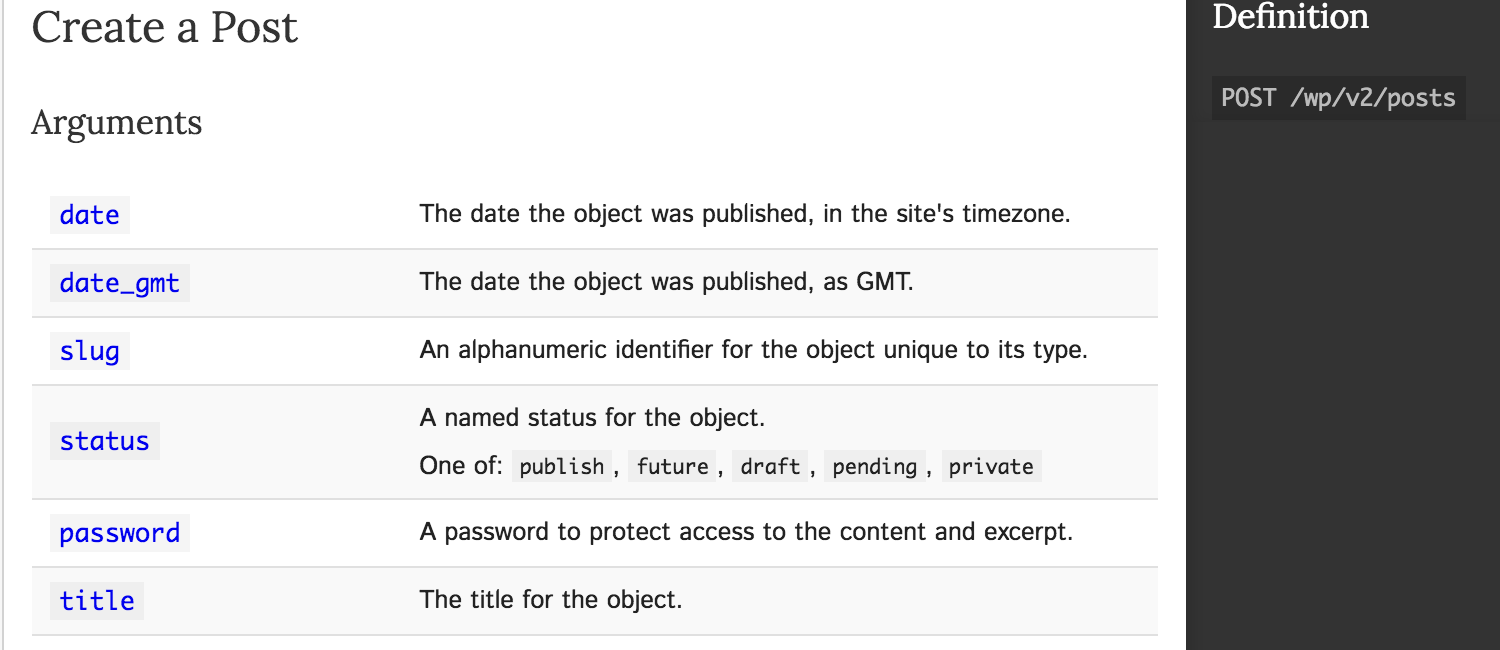
\includegraphics[width=\linewidth,height=2.5in,keepaspectratio]{original.png}}
\end{center}
\caption{Screenshot of the original WordPress REST API documentation}
\label{fig:original}
\end{figure*}

\begin{figure*}[tb]
\begin{center}
\fbox{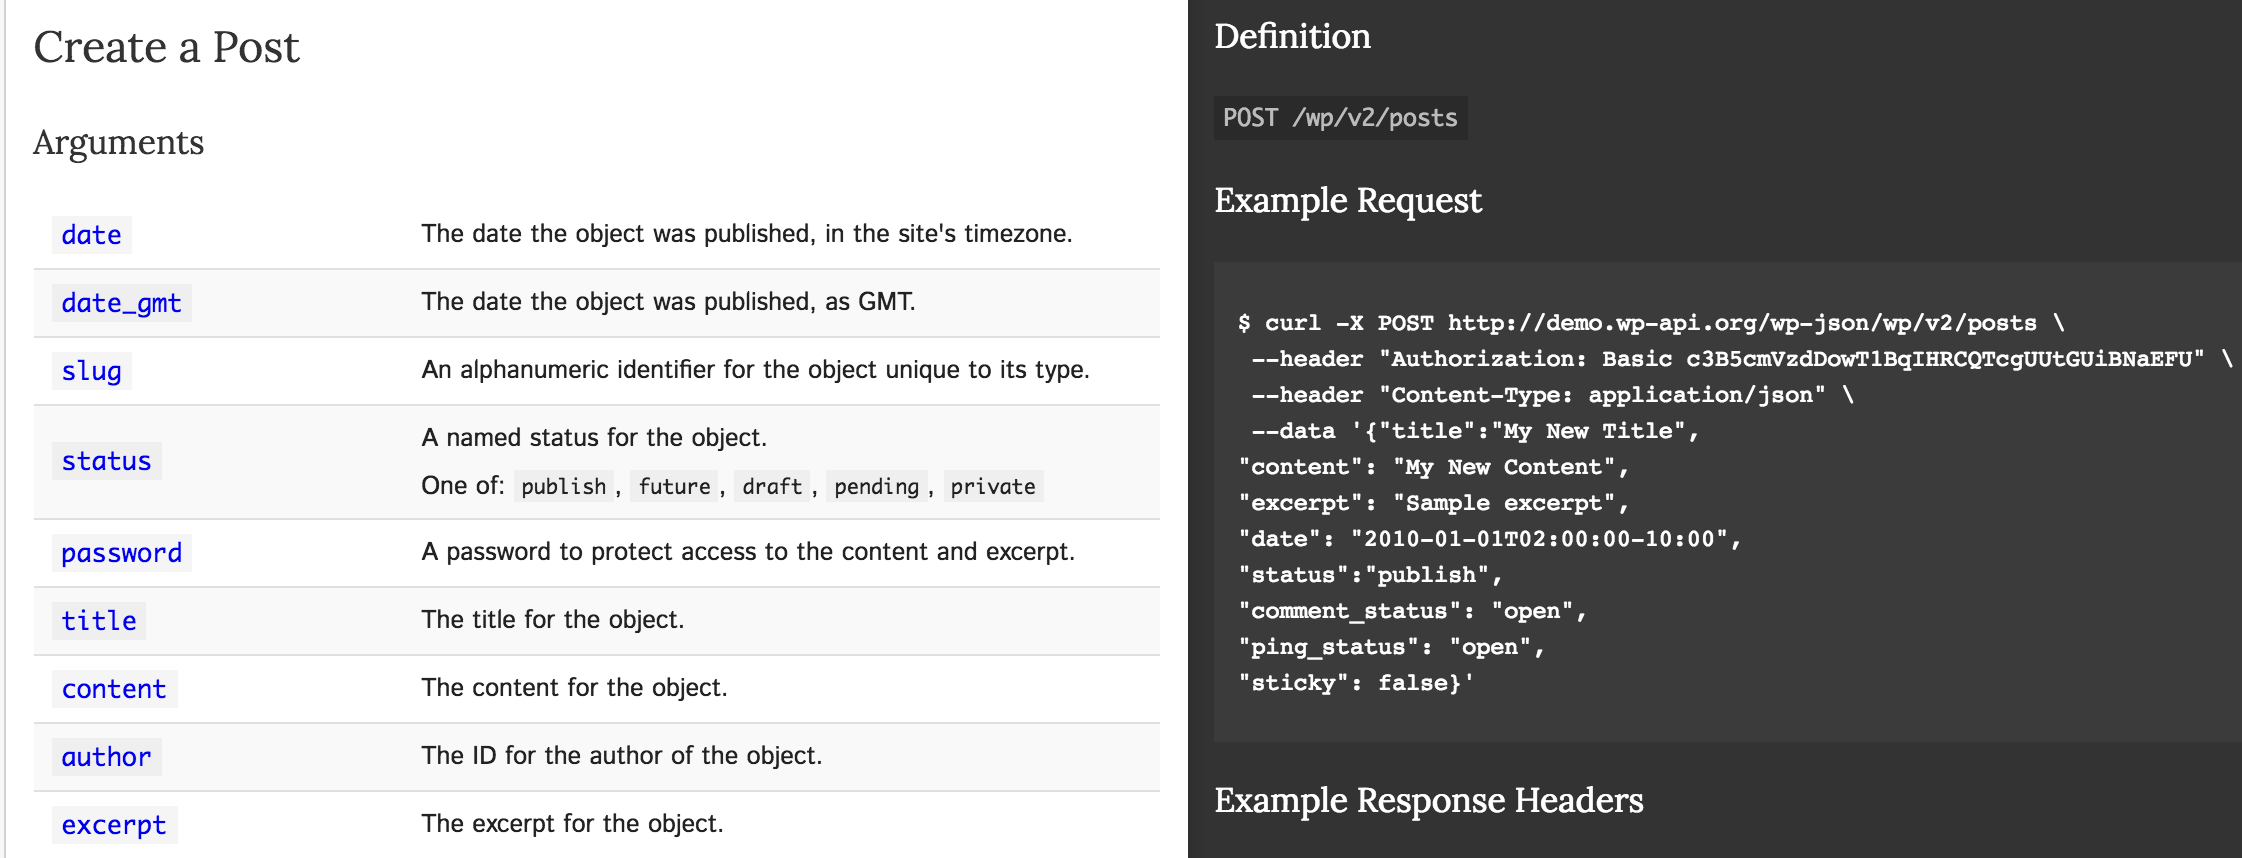
\includegraphics[width=\linewidth,height=2.5in,keepaspectratio]{forked.png}}
\end{center}
\caption{Screenshot of the forked WordPress REST API documentation with a usage example}
\label{fig:forked}
\end{figure*}


Based on the lessons learned from the pilot studies, we designed the actual study process as follows: the original WordPress REST API documentation was forked and a total of 3 API usage examples were added to show listing of blog posts with query parameters for filtering, a request to create a blog post and a request to update a blog post. Figure \ref{fig:original} shows a screenshot of the original API documentation related to T4 where the API client developers are provided with a reference table describing the different properties that can be used to create a $Post$ object\footnote{\url{http://v2.wp-api.org/reference/posts/}}. Figure \ref{fig:forked} shows a screenshot of the forked API documentation with a cURL based usage example. cURL is used because it's used by elsewhere in the original API documentation. In the forked API documentation, the example shows one possible API call with realistic values for the data that is described in the reference table and associated API response headers and body.

Participants were divided into two groups, G1 and G2. G1 participants were provided with a link to the official API documentation on the web-based API explorer, and G2 participants were provided with a link to the forked API documentation with usage examples. The web-based API explorer allocated more participants to G1 compared to G2 because we wanted to better understand the impact of the lack of usage examples on API client developer productivity. However, each individual participant was randomly assigned to a group by the web-based API explorer. All participants were given the same set of API tasks and were requested to limit their participation time to a maximum of one hour. No task specific time limit was imposed because we wanted participants to spend sufficient time on each task without forcing them to move the next one. Participants were allowed to access the internet and external resources alongside the provided API documentation to perform the tasks as they'd normally use on a typical work day.

\subsubsection{Data Collection} % (fold)
The data collected by the web-based REST API explorer for each participant is exported into a text file as the raw data artifact. For each API task and each participant that attempted the task, the exported text file contains the request inputs I1-4 and associated API response headers and body for each API call made by the participant. For each participant, we recorded all trial API calls with timestamps. Additionally, the demographic information, experience rating and the free-form feedback for each participant is also included in the artifact.


\subsubsection{Data Analysis}
The same data artifact is used to analyze both quantitatively and qualitatively to answer the aforementioned research question.We analyzed the data artifact qualitatively to understand the obstacles that REST API client developers face when using an API documentation that lacks usage examples. The data artifact exported from the web-based REST API explorer included a table with raw data. For each row, the table contains the following columns: API task, participant identifier, timestamp, API trial number, I1-4, response headers and body. It allowed us to observe and categorize the different input values that the participants used to perform the given API tasks. The values for I1-4 used by the participants were manually coded to group the participant responses into categories. The categories help us determine the types of information that API client developers need in the API documentation to perform API tasks successfully. The analysis started with an empty set of codes and new codes were introduced to describe scenarios that didn't fall under  codes that were already applied. The first author on this paper applied the codes on the raw data artifact and the co-authors verified the codes randomly. To resolve disagreements, the authors discussed and updated the codes accordingly. The codes were then further categorized to higher level grouping to represent common problems faced by the study participants for each group.

For each API task attempted by each participant, we annotated the artifact with one of the following labels: successful, partially successful, and unsuccessful. Task participations are marked successful when I1-4 matches the required values for performing the given task. If a participant is able to use the correct I1-4 for one of the two tasks required to complete a single task (T2), we marked it as a partially successful. Otherwise, it's marked as unsuccessful. Based on these annotations, the answers for RQ1 was computed using the following:


success rate of group = (total number of successful tasks by group) / (number of participants in group * number of API tasks)

API calls per success of group = (number of API calls annotated as successful) / (total number of trial API calls made by group)

average time taken for success = (number of successful API tasks by group) / (total time spent by all participants in the group)


\section{Results}
\label{sec:results}
\subsection{Qualitative Analysis Results} % (fold)

\textbf{Observation 1.} REST API client developers want usage examples along with the definition of API elements. From analyzing the participant feedback, we've observed usage examples mentioned as the most frequent and central topic of interest. 11 of the 16 G2 participants mentioned the lack of examples with HTTP headers, request and response as the primary problem with the API documentation. On the other hand, 7 out of the 10 G2 participants mentioned the examples being helpful from the forked documentation. This is also supported by our quantitative analysis as discussed later in this section.

\textbf{Implication 1.} REST API developers need to provide usage examples showing sample requests and responses with HTTP headers and body for API actions to help API usability.


\textbf{Observation 2.} API client developers face problem with using right data type without examples. To successfully complete T1 participants had to use an integer ID representing an $Author$ object given the author name. In the original API documentation, the following is mentioned about the author parameter: ``author: Limit result set to posts assigned to specific authors.'' The documentation doesn't mention that the data type required is the numeric author ID, not the author name. We found 10 of the 16 participants from G1 made API calls with the author name instead of the ID. P1.12 mentioned the following: \textbf{``...to find posts for the author, I had to inspect the response to see that indeed the $author\_id$ was in there''}. The forked documentation showed one example of using numeric ID. 3 of the 10 participants from G2 ran into the same error. When faced with this error, participants used trial and error to eventually complete the task.

\textbf{Implication 2.} REST API documentation needs to include examples of data types for each API field to satisfy API client developer information need.

\textbf{Observation 3.} API client developers face problem with using the right data format without examples. Tasks T3 required the use of a correct format to represent an array of numeric post IDs to be excluded using the API. The original documentation mentions the following about this API query parameter: ``exclude: Ensure result set excludes specific IDs.'' Participants attempted to solve this task using multiple different formats for specifying the array. For example: they tried with $exclude=[1,4]$, $exclude=1\&4$, $exclude=4\&\&exclude=1$, $id!=1\&id!=4$ and other alternatives before eventually finding the right format as follows $exclude=1,4$. Participant P1.6 mentioned the following: \textbf{``It was difficult to figure out whether some of the inputs needed to be arrays or just a comma-separated list.''} 7 out of the 16 participants in G1 faced this error. The forked documentation showed one example of using multiple IDs and all G2 participants could use the right format.

Task T5 also required the participants to use an ISO8601 formatted date for publishing a post with a specific date. Even though the documentation mentions ISO8601 format, it doesn't provide an example. So, participants had to use online search. P1.8 mentioned the following: \textbf{``Got hung up trying to figure out the formatting of the date (which doesn't appear to be ISO8601, despite what it says)''}. After analyzing the response, we found that P1.8 used the ISO8601 formatted date in the API calls, but didn't provide the $second$ portion of the time as required by the API. 8 of the 16 participants in G1 had an error in the date formats. With an example, 1 of the 10 participants had the same error from G2.

\textbf{Implication 3.} REST API developers need to include examples showing the valid data format for the API elements.


\textbf{Observation 4.} REST API client developers face problem with using request headers without usage examples. Tasks T5 and T6 required the use of a HTTP request header named $Content-Type$. In the original API documentation, the following was mentioned: ``The API uses JSON exclusively as the request and response format, including error responses.''. Experienced software engineers still had problem using this HTTP header as we found from the participants in G1. P1.12 mentioned the following: \textbf{``I didn't know how to specify application/json so that I could send POST data via the body instead in the URL parameters... Examples would really help - with a sample request and a sample response.''} We were surprised to see that 14 of the 15 participants that attempted T5 and T6 from G1 had the error of not specifying the $Content-Type$ header even though they have years of experience with REST APIs. In contrast, 2 out of the 10 participants from G2 failed used this header correctly as indicated in the example in the forked documentation. Moreover, 1 of the 2 G2 participants that didn't use the header first time, later used it correctly on a subsequent attempt.

\textbf{Implication 4.} If API requests need to use HTTP Request headers, in addition to the request method and body, REST API develpers need to include examples of the HTTP headers.

\textbf{Observation 5.} API client developers face problem with performing API tasks that require multiple API calls. Tasks T2 and T6 required the use of multiple API calls to complete successfully. Both tasks require an initial API call to find data using the API that is needed make a second API call. For example, P1.5 mentioned the following about T6, \textbf{``The post I created is not visible and not editable, though I got 201. Not sure why''}. After analyzing the response, we observed that P1.5 was able to create a blog post, but failed to publish it because it didn't have the $publish$ status. As a result, the post was not returned via the API for T6. P2.2 mentioned the following about T2: \textbf{``In case of search posts by author, it's not clear how to find the author\_id. Although, I realized that users and authors are same in this case.''}

\textbf{Implication 5.} If there are prerequisites for making an API call, REST API developers need to provide examples showing how to get the prerequisites in the API documentation.


To summarize, we recommend API developers to consider usage examples as an essential requirement for REST API documentation. As such, sufficient resources and a high priority should be devoted to generate and maintain the usage examples. Based on our observations, we recommend REST API documentation tools to provide first-class support for including usage examples with realistic data.

\subsection{Quantitative Analysis Results} % (fold)

\pgfplotsset{compat=1.14}
\usetikzlibrary{patterns}
\pgfplotstableread[col sep=comma]{groupone.csv}\groupone

\begin{figure*}

\centering

\begin{subfigure}{0.5\textwidth}
\centering
\begin{tikzpicture}
    \begin{axis}[
        ybar,
        xtick=data,
        xticklabels from table={\groupone}{Task},
        legend style={at={(0.5,-0.15)},
        anchor=north,legend columns=-1},
        ylabel=Average Trial API Calls,
        width=2.8in
    ]
    \addplot[pattern=crosshatch dots, pattern color=gray] table [col sep=comma, x expr=\coordindex, y=AverageAPICalls] {groupone.csv};
    \addplot[draw=black] table [col sep=comma, x expr=\coordindex, y=AverageAPICalls] {grouptwo.csv};
    \legend{G1: Using Original, G2: Using Forked}
    \end{axis}


    \begin{axis}[
      axis y line*=right,
      axis x line=none,
      ymin=0, ymax=100,
      ylabel= Success Rate,
      yticklabel={\pgfmathparse{\tick}\pgfmathprintnumber{\pgfmathresult}\%},
      width=2.8in,
      legend style={at={(1.0,1.25)},anchor=north east},
    ]
    \addplot[dashed,mark=*,gray] table [col sep=comma, x expr=\coordindex, y=SuccessRate] {groupone_success.csv};
    \addlegendentry{G1: Using Original}

    \addplot[smooth,mark=*,black] table [col sep=comma, x expr=\coordindex, y=SuccessRate] {grouptwo_success.csv};
      \addlegendentry{G2: Using Forked}
    \end{axis}
\end{tikzpicture}
\caption{Trial vs. Successful API Calls}
\label{graph:productivity}
\end{subfigure}
\begin{subfigure}{0.4\textwidth}
\centering
\begin{tikzpicture}
    \begin{axis}[
        ybar,
        xtick=data,
        xticklabels from table={\groupone}{Task},
        legend style={at={(0.5,-0.15)},
        anchor=north,legend columns=-1},
        ylabel=Average Time Spent (minutes),
        width=2.8in
    ]
    \addplot[pattern=crosshatch dots, pattern color=gray] table [col sep=comma, x expr=\coordindex, y=Time] {groupone_time.csv};
    \addplot[draw=black] table [col sep=comma, x expr=\coordindex, y=Time] {grouptwo_time.csv};
    \legend{G1: Using Original, G2: Using Forked}
    \end{axis}

\end{tikzpicture}
\caption{Average Time Spent}
\label{graph:time}
\end{subfigure}


\caption{Quantitative Comparison between G1 and G2}
\label{fig:comparison}
\end{figure*}

We present a summary of the quantitative results as found by analyzing a total of 539 API calls (385 from G1, 152 from G2) made by the participants from this study in Figure \ref{fig:comparison}. Figure \ref{graph:productivity} juxtaposes the average number of trial API calls made by each group against their rate of success in performing the given tasks T2-T6. The average number of trial API calls and success rate for each group is computed using the following formulas:

AverageTrialAPICall(task, group) = Total number of API calls made by group on task / Number of participants in group

SuccessRate(task, group) = Number of participants that correctly completed task / Number of participants in group

In Figure \ref{graph:productivity} and  \ref{graph:time} we see that, for the simpler tasks T2 and T3, G1 had used more trial API calls and more time on average and reached successful answers with a lower percentage compared to G2. For T4, where the participants are required to inspect a HTTP response header, G2 needed more API calls on average, but also yielded 24\% higher success rate. For the more complicated tasks T5 and T6, we see that participants in G1 had very low success rate and very high number of average API trials compared to G2. The data here clearly depicts that without usage examples REST API client developers spend more time and require more trial and error attempts yet resulting in lower success rates, and the situation gets worse for relatively complicated tasks.

\begin{figure}[h]
\centering

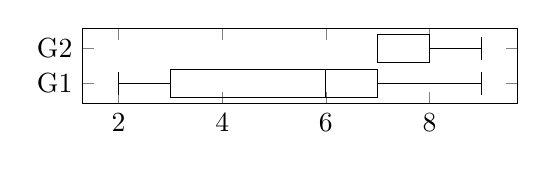
\begin{tikzpicture}
  \begin{axis}
    [
    ytick={1,2,3},
    yticklabels={G1, G2},
    width=2.8in,
    height=1in
    ]
    \addplot+[
    boxplot prepared={
      median=6,
      upper quartile=7,
      lower quartile=3,
      upper whisker=9,
      lower whisker=2
    }, color=black
    ] coordinates {};
    \addplot+[
    boxplot prepared={
      median=7,
      upper quartile=8,
      lower quartile=7,
      upper whisker=9,
      lower whisker=7
    }, color = black
    ] coordinates {};
  \end{axis}
\end{tikzpicture}
\caption{Participation Satisfaction Ratings on a Scale of 0-10}
\label{fig:rating}

\end{figure}

In Figure \ref{fig:rating}, we see that the G2 participants provided higher satisfaction rating compared to G1 participants. P1.1 provided a satisfaction rating of 9, and analyzing the participant feedback against the success, we see a false positive case, where the participant perceived that the tasks were successfully completed even though only 2 of the 5 tasks were correctly answered. Other than this case, the satisfaction ratings provided by G1 participants consistently fall behind the G2 participants' ratings.

Based on these results, we recommend REST API developers to study the usability of their API documentation with prospective API client developers and provide required usage examples in the documentation to improve API client developer productivity and satisfaction.


\section{Threats to Validity}
\label{sec:threat}
  The selection of the API, the tasks, and the participants may introduce selection bias. We have developed and followed a set of requirements as discussed earlier on this paper to reduce this bias. This study needs to be replicated with different sets of APIs, tasks, and participants to generalize the results. The analysis of the raw data may introduce a bias. To reduce this, we have involved multiple researchers in the analysis process.


\section{Related Work}
\label{sec:related_work}
\subsubsection{API Learning Obstacles}
  Researchers have published several papers on the topic of API learning obstacles. Robillard et al. used a mixed approach of surveys and in-person interviews with professional software engineers to understand the API learning obstacles \cite{Robillard_what_makes} \cite{Robillard_a_field_study}. They found that API documentation was related to one of the most severe obstacles for API learnabilty and recommended considering five factors for API documentation as follows: documentation of intent, code examples, matching APIs with scenarios, penetrability of the API, and format and presentation. Gias et al. surveyed 323 professional software engineers to understand the factors that fail a API documentation \cite{g_uddin}. They identified ambiguity, incompleteness, and incorrectness as the three severest problems that lead API documentations to fail to answer the information needs of developers. Duala-Ekoko et al. performed a study with twenty programmers to understand the types of questions that developers have while using an unfamiliar API \cite{Duala-Ekoko:2012:AAQ:2337223.2337255}. They categorized the API related information needs into twenty generic questions that can be used to analyze the quality of API documentation. Myers et al. performed a study of enterprise SOA API usability and found that the study participants had limited success finding the relevant API elements to perform an API task \cite{Myers_study}. Among other factors, they recommended providing code examples in the API documentation to help API client developers with sample solutions to different patterns of API tasks.

  In this paper, we focused on the usage examples part of API documentation to further understand the obstacles that API client developers face when the documentation contains relevant information about the API, it's intent, description of the API actions and elements, but lacks code examples.

\subsubsection{Crowd-Sourced API Usage Examples}
Several existing research has focused on sourcing API usage examples from the Internet. Wang et al. performed an exploratory study to understand the current state of API related knowledge available on the Internet that can be leveraged by API client developers \cite{6462686}. They searched the web for usage examples related to the API of five popular Java libraries and found that on an average API examples could be found for 77\% of the 4,637 APIs included in the selected libraries. Moreover, they found that the crowd-sourced API documented accounted for 93.7\% of the usage examples compared to 6.13\% that were published on the official documentation. Incorporating a corpus of crowd-sourced API examples from the web and using placeholders for commonly related API elements, an evaluation of Jadite found that developers were three times faster to complete API tasks \cite{5295283}. Nasehi et al. analyzed StackOverflow threads to understand the characteristics of good and bad code examples based on user provided votes \cite{Nasehi_what_makes}. They found that commonly down-voted API related answers lacked code examples, explanations, and shortcoming of solutions. They recommended API developers to evolve the documentation with usage examples to answer API client developer questions that were not anticipated in the existing documentation. Treude et al. proposed a machine learning based approach to find relevant API documentation from StackOverflow using both the text and metadata found from the questions and answers \cite{Treude:2016:AAD:2884781.2884800}. Kim et al. presented a technique to automatically augment code examples from the web using code search tools to Java APIs \cite{Kim:2009:AEJ:1747491.1747552}. Jiau et al. observed a severe inequality within the context of crowd-sourced API usage examples where most of the content were related to the popular APIs \cite{jiau}.

Existing research on crowd-sourced API documentation has mostly focused finding crowd-sourced usage examples of local APIs. In this paper, we focused on the impact of usage examples for REST APIs, where the API client development programming language is agnostic to the language used to implement the API. This important distinction with local APIs makes it hard to leverage the techniques proposed in the aforementioned papers to find relevant REST API usage examples.

\subsubsection{Measuring API Usability}
Several papers have been published on the topic of measuring API usability. Rama et al. presented a set of formulas for computing a measure of API usability based on the API's structural components such as classes, methods, parameters, return values, thread-safety, etc \cite{rama}. Scheller et al. presented a framework for automatically measuring the complexity of an API \cite{scheller2015automated}. They identified a list of measurable API properties and provided formulas to compute complexities related to the interfaces, implementation and setup of an API. Grill et al. proposed an HCI based approach that can be used by API developers to understand and improve on the problem areas related to an API \cite{Grill2012}. They suggested using a combination of expert opinion and developer workshops on APIs to identify and collect feedback about API and its documentation related problems. To improve API usability, Farooq et al. proposed using peer reviews of API code in addition to API usability studies to uncover API related bugs and incorporate feedback regarding the API elements \cite{Farooq:2010:AUP:1753326.1753677}. In our work, instead of measuring overall API usability, we have focused specifically on the relationship of REST API usability with respect to usage examples.

\subsubsection{Controlled Studies}
Several authors published the results of controlled studies on the topic of API usability. Nasehi et al. performed a controlled study to understand if API unit tests can be used to provide as usage examples to facilitate API client developers \cite{5609553}. They grouped participants into two groups, and one of the groups was provided with API unit tests in addition to the documentation. The two groups performed the same set of API tasks. The researchers found that the examples from the unit tests helped understanding the API concepts better but it was challenging for the participants to locate relevant examples from the corpus of unit tests. They recommended automated extraction of relevant high-level API usage examples from API unit tests. Endrikat performed a controlled study with four groups of participants to understand the impact of API documentation on APIs that are implemented using programming languages with static and dynamic type systems \cite{Endrikat:2014:ADS:2568225.2568299}. Participants were given a set of failing unit tests and were asked to make them pass by writing code using the studied API. They defined the API client developer productivity in terms of the time to get the tests passing. They found that the participant group using a statically typed API with explicit documentation were more productive than the other groups. Ellis et al. performed a controlled study with two groups of Java developers to understand the impact of using a constructor vs. a factory method design pattern on API client development time \cite{Ellis:2007:FPA:1248820.1248863}. They found that API client developers needed more time to complete API tasks when the API requires the use a factory method to instantiate objects compared to using a constructor.

Our work in this paper is based on a controlled study and shares part of the setup that were used by the aforementioned API related controlled studies with the following differences: our goal is to understand the obstacles faced by API client developers without usage examples;  we focus on REST APIs instead of a local API; and, the participants are professional software engineers.

\section{Conclusion}
In this paper, we presented a set of problems that experienced REST API client developers face while performing API tasks using API documentation that lacks usage examples. We identified that, without examples, REST API client developers have trouble using the correct data types, correct data formats, and required HTTP headers and request body. We've also presented empirical evidence that adding usage examples it is possible to reduce mistakes, improve success rate and developer satisfaction of using the API. Practitioners can follow our guidelines while documenting REST APIs to improve API usability.

\section*{Acknowledgment}

\bibliographystyle{IEEEtran}
\bibliography{IEEEabrv,refs}


\end{document}


